\documentclass[11pt,a4paper,oneside]{report}
\usepackage{setup}
\usepackage{setspace}
\onehalfspacing
\setlength{\parindent}{1.5em}
\setlength{\parskip}{0pt}
\captionsetup{font=small}

\begin{document}

% ------------------------------------------------
% Front matter
% ------------------------------------------------
\pagenumbering{gobble}

\begin{titlepage}
\thispagestyle{empty}
\centering

\vspace*{0.7cm}


\includegraphics[width=0.5\textwidth]{Figures/VU_Logo.png}

\vspace{1.6cm}

{\huge Master Thesis\par}

\vspace{0.7cm}
\noindent\rule{0.82\textwidth}{0.5pt}\par
\vspace{0.7cm}

{\Huge\bfseries An Agent-Based Model of CCP Systemic Risk: Client Clearing and Margin Procyclicality\par}
% Replace with final thesis title

\vspace{0.7cm}
\noindent\rule{0.82\textwidth}{0.5pt}\par

\vspace{1.2cm}

{\large by\par}
\vspace{0.5cm}

{\Large\bfseries Siddharth Yash Kukreja\par}
\vspace{0.3cm}
{\large (2902483)\par}

\vspace{1.6cm}

\begin{tabular}{rl}
\textit{Supervisor:} & Dr.\ Rex Wang Renjie\\
\textit{Second Assessor:} & Prof. Dr. Albert Menkveld \\
\end{tabular}

\vspace{1.6cm}

{\small
Submitted in partial fulfillment of the requirements for the\\
Master of Science in Finance - Honours Programme in Quantitative Finance.\\
Vrije Universiteit Amsterdam
\par}

% ------------------------------------------------
% Acknowledgements
% ------------------------------------------------

\vspace*{1.5cm}
\end{titlepage}

% \clearpage
% \pagenumbering{roman}

% \chapter*{Acknowledgements}
% \addcontentsline{toc}{chapter}{Acknowledgements}
% This thesis required the support of many others that begets acknowledgement. I'd like to thank Simudyne, and in particular Krishnen Vytelingum who took the time to discuss the model they created, offer advice throughout the process and aid me in my doubts. I would also like to thank my supervisor, Dr. Rex Wang who gave me the freedom and independence, and with it the trust, to explore a unique and challenging topic. I would also like to thank Prof. Theo Kocken who helped me develop my initial approach, introducing me to Agent-Based Models and the field of central clearing, and went above and beyond to offer his help. Finally, to Prof. Albert Menkveld\href{}{} who helped develop my interest in market microstructure and taught the theory that forms a large part of the market simulation, in addition to his work on central clearing.

\clearpage

% % ------------------------------------------------
% % Abstract + contents
% % ------------------------------------------------
% \clearpage
% \pagenumbering{roman}

% \chapter*{Abstract}
% \addcontentsline{toc}{chapter}{Abstract}
% This paper presents an Agent-Based Model for Central Clearing, including the understudied client clearing tier. The modelling of central clearing with a client tier through an Agent-Based Model is the first of its kind. It is built upon two layers: an exchange layer where fundamental, momentum, and noise traders put in orders on a Limit Order Book calibrated to reproduce the stylised facts of returns we see in empirical data; and a clearing layer where a Central Counterparty novates the trades placed on exchange, collecting margins and collateral and administering a default waterfall. The standard model is based on historical E-mini price data across a calm and a stressed period, and is then applied to study margin procyclicality. Simulations from the stressed model highlight the importance for non-bank clearing members to have an external source of funding, the inability to liquidate their own position to raise liquidity is a vulnerability. An observation made from the study of margin procyclicality is that higher constant margins do not remove risk, but relocate it from the client tier to the member tier. Members hit their capital limits and freeze the provisioning of clearing services, and the clients holding positions that they cannot exit end up defaulting. This highlights the importance for clients to have more than one clearing connection. An alternative model is later presented with stochastic and synthetic stressed paths, offering a calibrated ensemble of varied scenarios that can be employed for CCP systemic risk testing.

\clearpage
\tableofcontents
\clearpage

% ------------------------------------------------
% Main matter
% ------------------------------------------------
\pagenumbering{arabic}

\chapter{Introduction}\label{ch:intro}
- Post GFC growth of Central Clearing

- Pros of a CCP

- Concerns with CCP and Research

- Client Clearing

- ABM modelling

- Design  of my model

- Calibration

- What can you test from model - Hypotheses

- Contributions of paper

- Implications

\chapter{Related Literature}\label{ch:related}
% Sections only — \chapter{Related Work}\label{ch:related} is in main.tex.

\section{Clearing, Clients and Central Counterparties}\label{sec:rw-clearing}

 \cite{menkveld_vuillemey_2021} offer a systematic review of the theories and empirical studies on Central Clearing. They highlight a research questions that remain open for further work -- the workings of the client clearing market. Commodity Futures Trading Commission (CFTC) data indicates that as of January 2025, clients make up 73\% of margin posted at major CCPs, but despite this studies on client clearing remain scarce. \cite{ofr_2026} study client clearing and its implications for market structure and stability by looking at Credit Default Swaps. They find that the modal client has only a single clearing connection. In periods of stress, these dealers may also stop the provision of clearing services - cutting off their clients' access to CCPs. Based on this, the simplified ABM assigns each client to a single CM who can freeze the provision of clearing services.

\cite{galbiati_soramaki_2013} build a simplified and stylised network model of tiered CCP-clearer-client relationships. They find that tiering reduces CCP total exposure but concentrates it onto fewer, larger GCMs. These extreme exposures to the CCP become larger and less predictable, despite a reduction in the average large exposure. 
 \cite{borovkova_2013} find that while CCPs reduce systemic risk in homogeneous systems, the effect depends on the system's topology and degree of homogeneity. The model here is also heterogenous, clients and CMs vary in balance sheet sizes, anchored to realistic ranges. The assignment is relatively heterogenous, with some CMs carrying upto sixteen members and others carrying as little as three.


Contagion in the model is transmitted through a well documented mechanism. In stressful periods, leveraged institutions need to liquidate in volatile markets to meet margin calls and maintain capital ratios, leading to a procyclical spiral of further calls. \cite{thurner_2012} show that heavy tailed returns and clustered volatility arise from leverage and leverage limits and the liquidation of assets due to these constraints. \cite{aymanns_farmer_2015} further look at the dynamics of these leverage cycles, and find that countercyclical leverage rules dampen the cycle. \cite{bookstaber_2014} make use of an Agent-based model to study the effects of asset and funding based fire sales on financial vulnerability. Together, these papers establish the base of how contagion transmits through the model. CMs and clients have capital  constrains and may need to liquidate during stressful periods. 

\cite{haynes_mcphail_zhu_2019} further state that the Basel III leverage ratio serves as a likely binding constraint for derivative positions. \cite{acosta_smith_2018} further show that leverage ratio affected dealers reduce client clearing, restricting clients' access to central clearing. These elements motivate the capital constraints imposed on Bank and Non-Bank Clearing Members and their clients in the Agent-Based model, and how breaching these leads to a freeze of trading behaviour and client clearing services. 

\subsection{Margins and Procyclicality}

Through the advent of central clearing, risk does not disappear; counterparty risk is rather transformed into liquidity risk \citep{cont_2017}. Accounting losses in a bilateral system with Mark-to-Market changes turn into realised margin calls drawing on liquidity in central clearing. As risk-based margins rise with volatility, these margin calls are pro-cyclical \citep{brunnermeier_pedersen_2009} -- margins peak when funding is low, leading to a spiral which causes forced sales that further depress prices and lead to even more margin calls. \cite{glasserman_wu_2018} find that volatility spikes lead to destabilising margin calls in times of market stress. \cite{esrb_2020} report that at the start of the COVID-19 crisis, IM posted at the four largest EU/UK CCPs rose by a third of pre-crisis levels, daily VM calls at the same time quintupled on euro area investment funds' derivative exposures, and increases at this time stemmed mostly from client portfolios and to a lesser extent from house portfolios. Prompted by the large March 2020 margin calls, \cite{bcbs_cpmi_iosco_2025} set out to review CCP margining practices and created a policy proposal calling for greater transparency in margining practices by CCPs onto CMs and further onto clients. The stressful period used here is also calibrated on the COVID-19 onset data. 

 \cite{paddrik_rajan_young_2020} use CDS trade level data to model how a credit shock triggers margin calls through a network of members and clients. They find that large client firms in the periphery with imbalanced portfolios contribute most to contagion. Through this model, we also see that a few large client defaults overwhelm the CMs more than many small defaults. An alternative to margins that react to recent market volatility are "through the cycle" margin models that ask for higher margins in quiet times \citep{glasserman_wu_2018}. These additional requirements, also called anti-procyclicality tools, minimise destabilising increases in IM requirements during market stress \citep{blanck_2025}. We therefore look at how these constant through the cycle margins compare with reactive VaR based margining as a demonstrative test for our model.

\section{Agent-Based Models}

Analysis of CCP risk and practises can only go so far with historical data. Agent-Based modelling is a novel methodology to study complex, adaptive and emergent behaviours arising from the interactions of heterogeneous agents \citep{axtell_farmer_2025}, and through this it offers an excellent approach for the analysis of central clearing. The analysis of these behaviours is particularly useful when looking at stressed market environments, and ABMs have found increasing popularity in recent years in simulating financial markets. \cite{deloitte_ccp} develop an agent-based CCP risk model to analyse the effects of proposed recommendations to CCP risk practices laid out in a white paper by major global CMs \citep{ccp_path_forward_2020}, such as the adequacy of Cover-2 for CCP default funds. They incorporate a simulated market environment with an exchange and CMs, complete with a limit order book where CMs submit orders and exhibit behaviours found in fundamental, momentum and noise traders. The CCP then collects margins based on these trades, which each CM needs to answer, alongside a default management framework to simulate realistic CCP behaviour. The model in this paper is in many ways an extension of this model, adopting a similar architecture and extending it with a client tier.\footnote{The publicly available descriptions of this model are the
practitioner white paper \citep{deloitte_ccp} and Simudyne's online model
documentation; the detailed model documentation on which
Chapter~\ref{ch:model} draws was provided to the author by Simudyne and is cited as unpublished technical documentation \citep{simudyne_odd}.}

\subsection{Financial Market Simulations}

The first stage in the model is the design of a simulated market environment. The market simulations attempt to reproduce the stylised facts of returns we see in the market -- heavy tails, near zero autocorrelations and volatility clustering. One approach behind this is to look at price dynamics through linear price impact caused by the aggregate and excess demands of different trader agents. An early paper on this is \cite{chiarella_1992}, which populates the market with fundamentalists trading on a fundamental value and chartists trading on momentum and trend. An extension of this model is proposed by \cite{majewski_2018}, who add noise traders and allow for a long term drift in fundamental asset value and create an Agent-Based Model (Extended-Chiarella Model). In their model, the parameters carried by each trader are jointly estimated alongside the Fundamental Value using a Kalman Filter and an Expectation Maximisation algorithm. This offers inspiration for this paper, which calibrates the parameters of a synthetic Fundamental Value signal alongside agent parameters. 

Another approach replaces the aggregate price impact mechanism with an explicit limit order book (LOB) such that prices emerge from the matching of submitted orders. \cite{chiarella_iori_perello_2009} place fundamentalists, chartists and noise traders in such a system. \cite{farmer_2005} show that noise (Zero-Intelligence) traders submitting orders - limit orders, market orders, and cancellations - at random in a continuous double auction are adequate in explaining 96\% of variance in the bid-ask spread and 76\% of the variance of the price diffusion rate. \cite{cont_stoikov_talreja_2008} propose a stylised model for the dynamics of a limit order book, where order flows are governed by independent Poisson processes, separated into independent rates for market orders, limit orders and order cancellations. \cite{gao_2022_hfabm} construct a High Frequency ABM at millisecond levels to simulate the 2010 Flash Crash, and use a surrogate modelling technique to calibrate parameters.

The financial simulation in this paper is based upon these models, with a discrete time LOB operating at a 1-min frequency, populated by Fundamental Traders, Momentum Traders and Noise Traders. Fundamental Traders trade according to an exogenous fundamental value signal, Momentum Traders trade on a momentum signal and Noise Traders place orders at independent rates for market orders, limit orders and order cancellation. The model is calibrated on real market data and includes a calm and a stressed period to investigate resilience and margin procyclicality under stress.



\subsection{Model Calibration}

The credibility of an agent-based model is dependent on how well it is calibrated, i.e. how well it captures realistic behaviours. For the market simulation, the calibration approach used is a minimisation of distance from stylised facts of returns we see on the market. \cite{cont_2001} present a set of stylised facts for returns such as heavy tails, an absence of correlation, volatility clustering and a slow decay of autocorrelation in absolute returns. \cite{cont_2007} find that for agent-based models, volatility clustering in particular remains difficult to reproduce, and the ones that manage to do so include a switching of the market between high and low activity periods. 

To measure distance from these stylised facts, a loss function must first be defined that quantifies this robustly. \cite{franke_westerhoff_2012} calibrate a financial market simulation agent-based model by minimising the distance between simulated and empirical moments, by weighing each moment by the inverse of its sampling variability so that more weight is put onto less noisy moments. They construct a sample of these moments using a block-bootstrap approach on empirical data. They then validate these moments using moment specific p-values and a moment coverage ratio. Calibration of these moments can be computationally very expensive, as they require a full simulation of the model. \cite{lamperti_2018} address this by pioneering a surrogate modelling approach for the calibration of agent-based models. They train a machine learning surrogate - in this case an XGBoost model - to approximate parameter-to-loss mapping and use active learning to concentrate around the optimum. 

\cite{gao_2022_xgb} further extend this to an XGB-Chiarella approach to estimate the parameters of a Chiarella model. An XGBoost model is trained on a random sample of parameters to predict a loss function. \cite{gao_2022_hfabm} use this methodology to identify a promising region of parameters for their High Frequency Agent-Based market simulation and then perform a grid search around the region to obtain optimal parameters. The thesis makes use of this machine learning surrogate modelling approach to calibrate parameters and steer model design. We also apply this approach to jointly calibrate the parameters of a synthetic FV signal alongside the other parameters, a novel application that combines this calibration methodology with a precedence for joint calibration through \cite{majewski_2018}.

\chapter{Model Architecture: Client Clearing ABM}\label{ch:model}
% %==============================================================================
% %  CHAPTER 3 — MODEL STRUCTURE AND DESIGN
% %------------------------------------------------------------------------------
% %  Style: matches introduction.tex conventions (\citep/\citet authoryear; keys
% %  resolve against introduction_refs.bib + model_refs.bib). Calibration of the
% %  behavioural parameters is deliberately deferred to the Data & Calibration
% %  chapter; this chapter fixes the model's structure and cites the design
% %  source for every mechanism (Simudyne ODD first; deviations flagged inline).
% %==============================================================================
% The model is a discrete-time agent-based simulation of a centrally cleared
% futures market, built in two coupled tiers. The first tier is a
% \emph{market-microstructure layer}: a limit order book (LOB) on which
% heterogeneous traders exchange a single asset --- the E-mini S\&P~500 (ES)
% front-month future --- around an exogenous fundamental-value process derived
% from real ES data. The second tier is a \emph{central-clearing layer} placed
% on top of the first: a central counterparty (CCP), banking and non-banking
% clearing members, and a population of cleared end-clients, connected by the
% star topology of a real clearing system and governed by
% regulation-grounded margin, default-fund, and default-management mechanics.
% The architecture follows the Simudyne CCP Risk Model
% \citep{simudyne_odd,deloitte_ccp}, which this thesis extends in one central
% direction: the ODD's clearing members trade only for their own account,
% whereas here most market participants do not face the CCP directly but clear
% \emph{through} a member --- the client-clearing tier whose stress behaviour
% is the object of study. Throughout, the design rule is that every mechanism
% and constant is taken from a reference model, from regulation, or measured
% from data; where the implementation deviates from the primary reference, the
% deviation is stated and motivated.

% The two tiers are deliberately asymmetric in how their parameters are set.
% The market layer's behavioural parameters are \emph{calibrated} so that the
% simulated price reproduces the empirical stylised facts of ES returns
% \citep{cont_2001}; the calibration methodology and results are the subject
% of Chapters~4 and~5. The clearing layer contains no free behavioural
% parameters at all: margin rates, default-fund sizing, capital floors, and
% waterfall structure are pinned to their regulatory or reference values. The
% intention is that the clearing tier acts in a market environment that has
% been \emph{earned} from data rather than assumed, while the clearing
% mechanics themselves remain transparent and auditable.

% Time advances in one-minute steps over 6.5-hour regular trading sessions,
% the ODD-native cadence \citep{simudyne_odd}. Two market regimes are used
% throughout: a \emph{calm} regime (calendar year 2019) and a \emph{stressed}
% regime (the COVID-19 crash window, late February to early April 2020), each
% with its own fundamental path and its own calibrated parameter set.

% %==============================================================================
% \section{The market simulation}
% \label{sec:model-market}

% The trading venue is a single limit order book with price--time priority and
% a tick size of \$0.25 (the CME ES specification). Orders accumulate during
% each one-minute step and are crossed in a call auction at the step's end;
% executions print at the resting limit price. The mid-price
% $p_t = (b_t + a_t)/2$ is the average of the best bid and ask, falling back
% to the last traded price when one side of the book is empty. Resting orders
% leave the book only by execution or explicit cancellation: the fundamental
% and momentum traders manage a single standing order each by
% \emph{replace-on-new}, while zero-intelligence orders are cancelled
% stochastically at a per-order rate (Section~\ref{sec:model-agents}). This
% deviates from the ODD's blanket ten-step order lifetime, which was removed
% because it was redundant with --- and masked --- the explicit
% \citet{cont_stoikov_talreja_2008} cancellation rate that is the standard
% order-lifetime mechanism in this model class; the deviation is flagged
% against \citet{simudyne_odd}.

% The runtime population places $100$ agents on the book: $30$ fundamental
% traders, $10$ banking clearing members trading their own account with
% identical fundamental-trader logic, $20$ momentum traders, and $40$
% zero-intelligence traders. Off the book sit five non-banking clearing
% members and the CCP. Ninety of the LOB traders are \emph{cleared clients}
% who access the CCP only through a clearing member
% (Section~\ref{sec:model-margin}).

% %------------------------------------------------------------------------------
% \subsection{Trading agents}
% \label{sec:model-agents}

% Three behavioural types populate the book, the canonical
% fundamentalist--chartist--noise decomposition of the Chiarella family
% \citep{chiarella_1992,majewski_2018} in the LOB form of the Simudyne CCP
% model \citep{simudyne_odd}. All arrival decisions are per-step Bernoulli
% draws at the one-minute cadence, and order sizes are uniform,
% $q \sim \mathcal{U}\{1,\dots,10\}$ \citep{simudyne_odd}.

% \paragraph{Fundamental traders (FT).}
% Each fundamental trader $i$ holds a fixed idiosyncratic belief draw
% $z_i \sim \mathcal{N}(0,1)$ and forms, at every step, a reservation price
% around the fundamental value $V_t$:
% \begin{equation}
% \label{eq:ft-reservation}
% R_{i,t} \;=\; V_t + z_i \,\sigma^{f}_{t},
% \qquad
% \sigma^{f}_{t} \;=\; c_f\,\sigma_t\,v_0 ,
% \end{equation}
% where $\sigma_t$ is the prevailing local volatility of the fundamental
% (Section~\ref{sec:model-fv}), $v_0$ the regime's initial price level, and
% $c_f$ a calibrated scale governing the dispersion of beliefs --- the
% volatility-tracking belief width of the Deloitte specification
% \citep{deloitte_ccp}, which widens the reservation cloud in turbulent
% periods. The trader submits one limit order \emph{at} its reservation price
% on the side implied by its own mispricing,
% $\mathrm{sign}(R_{i,t} - p_{t-1})$, replacing any order it has standing.
% Because $z_i$ is persistent rather than redrawn, optimistic traders
% accumulate long inventories and pessimistic ones short inventories over
% time; this heterogeneous-beliefs specification
% \citep{chiarella_1992,majewski_2018} is load-bearing for the clearing tier,
% since margin calls and default management act on exactly these concentrated
% positions.

% \paragraph{Momentum traders (MT).}
% Each momentum trader tracks an exponentially weighted moving average of
% one-minute mid log-returns $r_t = \ln p_t - \ln p_{t-1}$,
% \begin{equation}
% \label{eq:mt-ewma}
% M_t \;=\; (1-\lambda)\,M_{t-1} + \lambda\, r_{t-1},
% \end{equation}
% and, whenever $|M_t|$ clears a small activation floor, posts a single
% passive limit order on the trend side at a stochastic depth of
% $k \sim \mathrm{Geom}(p_{\mathrm{zi}})$ ticks from the mid, managed
% replace-on-new. The trend horizon $\lambda$ is fixed by design rather than
% estimated, following \citet{majewski_2018}, who likewise impose the
% chartist timescale externally. Momentum traders are limit-only: an earlier
% market-order branch was removed because trend-chasing marketable flow
% corrupted the near-zero autocorrelation of simulated returns.

% \paragraph{Zero-intelligence traders (ZI).}
% The liquidity floor of the book is supplied by zero-intelligence traders in
% the tradition of \citet{farmer_2005} and \citet{cont_stoikov_talreja_2008}.
% In each step a ZI trader independently (i) cancels each of its resting
% orders with probability $\delta_{\mathrm{zi}}$, (ii) submits a limit order
% with probability $\alpha_{\mathrm{zi}}$ at a uniformly random side and a
% geometric depth $k \sim \mathrm{Geom}(p_{\mathrm{zi}})$ from the mid, and
% (iii) submits a market order with probability $\mu_{\mathrm{zi}}$, with no
% dependence on any signal. The placement parameter $p_{\mathrm{zi}}$ is not a
% free parameter: it is fitted by maximum likelihood to the depth distribution
% of new order arrivals in ES market-by-price (MBP-10) data, so the simulated
% book's near-mid thickness is anchored to the measured one. The arrival and
% cancellation rates are calibrated; the market-order rate is pinned at the
% \citet{cont_stoikov_talreja_2008} baseline.

% Two agent types that appear in related designs are deliberately absent. An
% always-quoting market maker \citep{gao_2022_hfabm} and a volatility trader
% \citep{gao_2023} were both implemented and removed after an ablation study
% showed the former damps volatility and clustering in both regimes while the
% latter helps only under stress; the ablation is reported with the
% calibration results.

% %------------------------------------------------------------------------------
% \subsection{The fundamental value process}
% \label{sec:model-fv}

% The fundamental $V_t$ is exogenous to the simulation: a path generated
% offline and read in as a time series, following the data-driven fundamental
% signal of the ODD \citep{simudyne_odd} and the data-derived fundamental of
% the XGB-Chiarella line \citep{gao_2022_xgb}. Two interchangeable generators
% are used, with distinct roles.

% \paragraph{Primary: the observed efficient price.}
% For the headline experiments the fundamental is extracted from the real ES
% one-minute mid by a local-level state-space model,
% \begin{equation}
% \label{eq:kalman}
% \ln V_{t+1} = \ln V_t + \mu + \sigma_v \varepsilon_t,
% \qquad
% \ln p^{\mathrm{obs}}_t = \ln V_t + \eta_t,
% \qquad
% \eta_t \sim \mathcal{N}(0, \sigma_\eta^2),
% \end{equation}
% estimated per session by Kalman maximum likelihood and smoothed by the RTS
% recursion, in the spirit of \citet{gao_2022_xgb} and of
% \citet{majewski_2018}, who treat the fundamental as a latent state filtered
% from price. One property of this construction is reported plainly: at the
% one-minute frequency the ES \emph{mid} contains almost no i.i.d.\
% microstructure noise (the noise that model \eqref{eq:kalman} is built to
% remove lives in trade prices, not in quote midpoints), so the estimated
% $\sigma_\eta$ is of order $10^{-5}$ and the smoother is near-identity. The
% fundamental is therefore, in effect, the observed efficient mid --- the
% Kalman step \emph{verifies} that mid-price noise is negligible rather than
% delivering material smoothing --- and the simulated market inherits the real
% return tails through $V_t$, which the agent layer must transmit and reshape
% rather than manufacture from nothing. Two features of the construction
% matter for the clearing tier. First, the per-session series are concatenated
% at their true levels, so \emph{overnight gaps are retained}: the COVID
% episode carries its actual peak-to-trough drawdown of roughly $-33\%$, most
% of which occurred between sessions. The simulator opens each session by
% repricing the entire book at the gapped fundamental, a clean between-session
% jump that stresses the cleared positions without contaminating intraday
% returns. Second, a per-minute local volatility
% $\sigma_t = \sqrt{\mathrm{EWMA}[r^2_t]}$ accompanies the path and drives the
% fundamental traders' belief width in \eqref{eq:ft-reservation}.

% \paragraph{Scenario generator: a stochastic-volatility jump diffusion.}
% For Monte-Carlo experiments that require many independent stress episodes, a
% synthetic alternative generates $V_t$ as a geometric diffusion whose
% volatility mean-reverts as an Ornstein--Uhlenbeck process
% \citep{stein_stein_1991,heston_1993}, overlaid with compound-Poisson jumps
% \citep{merton_1976} and with empirical overnight gaps:
% \begin{align}
% \sigma_{t+1} &= \theta + e^{-\alpha}(\sigma_t - \theta) + s\,\varepsilon^\sigma_t,
% \label{eq:svmjd-vol}\\
% \ln V_{t+1} - \ln V_t &=
% \begin{cases}
% \mu + \sigma_t \varepsilon_t + J_t, & J_t \sim \mathcal{N}(0,\delta^2)
% \text{ w.p. } \lambda/390, & \text{(intraday steps)}\\[2pt]
% G_t \sim \widehat{F}_{\mathrm{on}}, & & \text{(session boundaries)},
% \end{cases}
% \label{eq:svmjd-ret}
% \end{align}
% where $\widehat{F}_{\mathrm{on}}$ is the empirical distribution of the
% regime's observed overnight returns, resampled nonparametrically. Every
% parameter of \eqref{eq:svmjd-vol}--\eqref{eq:svmjd-ret} is measured from the
% ES data with standard realized-measures estimators rather than assumed: the
% diffusion variance from jump-robust daily bipower variation
% \citep{bns_2004}, the jump intensity from threshold exceedance counts
% \citep{mancini_2009} --- approximately $1.9$ per day in the calm regime and
% $1.0$ per day under stress, superseding the FTSE-based intensity of the ODD,
% a flagged deviation --- and the jump size from the realized-variance minus
% bipower-variation jump component, whose share of intraday variance
% ($6.8\%$ calm, $3.9\%$ stressed) sits on the $5$--$7\%$ benchmark
% established for the S\&P~500 \citep{huang_tauchen_2005}. The
% Ornstein--Uhlenbeck parameters are fitted to a jump-robust intraday
% volatility series with noise-robust autocovariance moments, and the
% long-run level $\theta$ is re-anchored so the stochastic-volatility layer
% redistributes, rather than inflates, the measured variance. The overnight
% component is included because gaps carry roughly $40\%$ of ES close-to-close
% variance in both regimes and because the COVID decline itself was
% concentrated overnight while intraday returns netted positive --- the
% overnight/intraday asymmetry documented by \citet{lou_polk_skouras_2019}.
% Stressed episodes default to the empirical window length of $29$ sessions,
% so that a ``stressed scenario'' means an episode of COVID-like length and
% severity rather than an indefinitely compounded crash.

% %==============================================================================
% \section{The margin framework}
% \label{sec:model-margin}

% The clearing tier connects the market to a single CCP through the star
% topology of \citet{simudyne_odd}: every clearing member holds a bilateral
% link to the CCP, which becomes the counterparty to all cleared positions
% upon novation. Two member types are distinguished, as in the ODD. A
% \emph{banking clearing member} (BCM) trades its own account --- with
% fundamental-trader logic, so the market-layer calibration is unaffected by
% the cast --- and additionally guarantees a book of clients. A
% \emph{non-banking clearing member} (NBCM) is a pure intermediary with no
% proprietary position; its entire balance-sheet capacity is client clearing.
% The thesis extension is the client tier itself: ninety end-clients
% (fundamental, momentum, and zero-intelligence types) clear through the ten
% client-carrying members in skewed books of five to fifteen clients, with the
% non-banking members carrying the largest books. Loss-absorbing capital is
% initialised at regulatory scale --- bank-level capital for BCMs, the
% non-bank futures-commission-merchant range for NBCMs, and entity-type-scaled
% cash for clients --- taken from CFTC member financial data and CCP
% disclosures.

% \paragraph{Variation margin.}
% Every 60 minutes the margin cycle marks each cleared book to the prevailing
% mid and settles the move in cash. Settlement is computed against
% \emph{average filled prices}, the ODD's margin-call profit-and-loss
% convention \citep{simudyne_odd}: writing $N_\tau$ for the end-of-cycle
% position, $m_\tau$ for the mark, and $\{(q_k, p_k)\}$ for the fills executed
% during the cycle,
% \begin{equation}
% \label{eq:vm}
% \mathrm{VM}_\tau \;=\;
% \Bigl[\, N_\tau\,(m_\tau - m_{\tau-1})
% \;+\; \textstyle\sum_k q_k\,(m_{\tau-1} - p_k) \Bigr]\cdot \ell \cdot \chi ,
% \end{equation}
% where $\ell$ is the per-regime contract lot that maps model volume to
% empirical ES volume and $\chi = \$50$ per index point is the CME multiplier.
% The second term in \eqref{eq:vm} settles each trade from its execution
% price, so that the slippage of forced liquidations
% (Section~\ref{sec:model-default}) is borne in cash by the liquidating party
% rather than lost between marks. Cleared participants use futures-style
% accounting throughout: a fill moves only the position, and cash moves only
% through the margin cycle.

% \paragraph{Initial margin.}
% Initial margin is charged on gross exposure as a value-at-risk scan --- for
% a single linear future, the SPAN scanning charge coincides with parametric
% VaR --- per EMIR's requirements for exchange-traded derivatives
% \citep{emir_rts}:
% \begin{equation}
% \label{eq:im}
% f^{\mathrm{IM}}_\tau \;=\;
% \max\!\Bigl( f_{\mathrm{floor}},\; z_{99}\,\hat\sigma^{\mathrm{day}}_\tau
% \sqrt{h} \Bigr),
% \qquad
% \mathrm{IM}_\tau = f^{\mathrm{IM}}_\tau \cdot
% \bigl(\,|N^{\mathrm{own}}_\tau| + \textstyle\sum_{c}|N^{c}_\tau|\,\bigr)
% \cdot \ell\,\chi\, m_\tau ,
% \end{equation}
% with $z_{99}$ the 99\% normal quantile, $h = 2$ days the margin period of
% risk, and an anti-procyclicality floor $f_{\mathrm{floor}}$ anchored to the
% CME's ES margin scale. The driving volatility $\hat\sigma^{\mathrm{day}}_\tau$
% defines the \emph{margin regime}, the experimental lever for the
% procyclicality hypothesis: in the \emph{reactive} baseline it is an
% exponentially weighted estimate of realised intraday simulation returns
% (half-life two sessions), so margin ratchets upward through a crash exactly
% as CME's ES margin was raised repeatedly through March 2020; a \emph{static}
% variant fixes it at the regime constant; and a \emph{flat} variant removes
% the volatility response altogether, charging a constant fraction --- the
% through-the-cycle comparator contemplated by the anti-procyclicality
% options of EMIR and the post-2020 margin debate
% \citep{murphy_2014,esrb_2020}. A maintenance threshold at $95\%$ of initial
% margin flags margin calls when a cycle's variation margin exceeds the
% remaining buffer \citep{simudyne_odd}.

% \paragraph{Capital adequacy.}
% Each member's capital ratio is cash over initial margin,
% \begin{equation}
% \label{eq:capital}
% \kappa_\tau \;=\; \frac{C_\tau}{\mathrm{IM}_\tau} \;\geq\; 8\%,
% \end{equation}
% the futures-commission-merchant net-capital rule, which sets required
% capital against \emph{risk margin} rather than gross notional
% \citep{cftc_reg117}. The distinction matters operationally: an FCM clears
% many multiples of its capital in client notional, so a notional-based floor
% would bind permanently, whereas \eqref{eq:capital} binds only as distress
% approaches. A banking member's proprietary book is additionally capped by a
% trading-book VaR limit, $|N^{\mathrm{own}}|\,\ell\chi m \leq
% \beta C / (z_{99}\hat\sigma^{\mathrm{day}})$ with $\beta = 5\%$ of capital,
% in the spirit of regulatory trading-book risk limits \citep{basel_frtb};
% without it, the fundamental-trader logic accumulates unbounded prop
% positions in a trend.

% \paragraph{Client clearing.}
% Each client carries its own balance sheet. The margin cycle issues every
% client its own variation-margin call, paid from the client's own cash and
% relayed by its member to the CCP; the client's live inventory is novated
% into the member's cleared book each cycle. A client can open positions only
% up to its broker house margin --- a fixed $20\%$ of notional, i.e.\
% five-times leverage, the conservative house multiple above the exchange
% minimum --- and is frozen (barred from new risk) when its cash falls below
% $8\%$ of its gross notional. Cash exhaustion is a client default and hands
% the position to the member (Section~\ref{sec:model-default}). This
% client tier is the thesis's central extension of the reference model;
% its empirical motivation --- clients supply the majority of margin at major
% CCPs and typically depend on a single clearing agent --- is documented by
% \citet{ofr_2026}.

% %==============================================================================
% \section{The default management framework}
% \label{sec:model-default}

% Default management proceeds in three escalating stages --- client default,
% member distress, member default --- and is closed by the CCP's prefunded
% resources. All liquidations use the same execution schedule: a position of
% size $X$ unwound over horizon $H$ follows the closed-form
% \citet{almgren_chriss_2000} trajectory
% \begin{equation}
% \label{eq:ac}
% \frac{x_j}{X} \;=\; \frac{\sinh\bigl(\kappa (H - j)\bigr)}{\sinh(\kappa H)},
% \qquad j = 0,\dots,H,
% \end{equation}
% with urgency $\kappa H = 2$ and $H = 30$ minutes, executed as market orders
% on the simulated book --- so liquidation impact is endogenous: the fire-sale
% walks the very book on which surviving members are marked, which is the
% price-mediated contagion channel of the model
% \citep{simudyne_odd,vytelingum_2025}.

% \paragraph{Client default.}
% A client whose cash is exhausted by variation margin defaults. Its member
% covers the uncollected margin call, assumes the client's position onto its
% own book, and liquidates it by \eqref{eq:ac} --- a banking member through
% its own orders, a non-banking member through orders routed by the CCP on its
% behalf. Because variation margin settles against fill prices
% \eqref{eq:vm}, the close-out loss is realised as the fire-sale walks the
% price: the member's loss is the deficit the liquidation actually produces,
% not a stylised haircut. This client$\to$member loss assumption is the first
% link of the cascade under study.

% \paragraph{Member distress.}
% A member breaching the capital floor \eqref{eq:capital} while still solvent
% acts before defaulting, asymmetrically by type as in the ODD
% \citep{simudyne_odd}: a banking member \emph{deleverages}, selling its
% proprietary book down by \eqref{eq:ac} until the floor is restored; a
% non-banking member, having no own book to sell, \emph{stops out} ---
% suspending new client risk, which freezes its clients --- for as long as the
% breach persists. The stop-out is state-based: it lifts if the ratio
% recovers. These are the liquidity-withdrawal behaviours that couple margin
% pressure back into the market layer.

% \paragraph{Member default and the waterfall.}
% A member whose cash is exhausted defaults. The CCP absorbs the member's
% realised cash deficit --- the shortfall it owes but cannot pay --- through
% the five-level waterfall of the reference model \citep{simudyne_odd}, in
% EMIR's defaulter-pays ordering \citep{emir_rts}:
% \begin{equation}
% \label{eq:waterfall}
% \text{L1 own DF contribution}
% \;\to\; \text{L2 CCP skin-in-the-game}
% \;\to\; \text{L3 pooled DF}
% \;\to\; \text{L4 survivors' cash}
% \;\to\; \text{L5 CCP capital}.
% \end{equation}
% The defaulted member is then removed from the system (ODD step sequence).
% Its surviving clients are \emph{ported}: each is reassigned to a surviving
% client-carrying member with spare risk capacity, accepted only if the
% receiver remains above its capital floor with the transferred book ---
% porting is the regulatory first option on a member default
% \citep{emir_rts}, but it is capacity-checked rather than guaranteed, since
% in practice the modal client has no standing backup agent
% \citep{ofr_2026}; clients that cannot be placed are closed out and
% deactivated. The member's own book, together with any unported client
% positions, passes to the CCP, which disposes of it by \eqref{eq:ac} on the
% open market. The CCP carries this book in a disposal account marked through
% the margin cycle: disposal-period losses re-enter the waterfall
% \eqref{eq:waterfall} of the originating default, so the mutualised loss is
% the close-out loss actually realised, symmetric with the client treatment.
% The open-market disposal is a flagged deviation from the ODD, whose default
% positions are auctioned to the surviving member with the largest opposing
% position; the deviation is deliberate, as the endogenous price impact of
% disposal is precisely the contagion mechanism the thesis measures.

% \paragraph{The default fund.}
% The mutualised layers of \eqref{eq:waterfall} are prefunded. The fund is
% sized daily to the \emph{cover-two} standard --- sufficient for the
% simultaneous default of the two largest members
% \citep{emir_rts} --- by the stress-loss-over-initial-margin method of
% Euronext Clearing \citep{euronext_a9}:
% \begin{equation}
% \label{eq:df}
% \mathrm{DF}_\tau \;=\; (1+b) \sum_{j \in \text{top-2}}
% \max\Bigl( 0,\; \bigl(s_\tau - f^{\mathrm{IM}}_\tau\bigr)\,
% |N_{j,\tau}|\,\ell\,\chi\,m_\tau \Bigr),
% \qquad
% s_\tau = \max\bigl(15\%,\; z_{s}\,\hat\sigma^{\mathrm{day}}_\tau\sqrt{h}\bigr),
% \end{equation}
% the loss each member would suffer beyond posted margin under an
% extreme-but-plausible move $s_\tau$, with buffer $b = 10\%$. The CCP
% prefunds a skin-in-the-game share ahead of the pooled fund, consumed at L2
% before any survivor resources \citep{simudyne_odd}; the EMIR skin-in-the-game
% rule is expressed against CCP regulatory capital rather than fund size, so
% the model's fund-share convention is a stylised assumption and is disclosed
% as such. Member contributions are paid \emph{in cash} into the fund, pro
% rata to exposure, and every post-draw daily recomputation is therefore a
% replenishment cash call on survivors --- the margin-liquidity channel that
% made the March 2020 episode a funding event as much as a solvency one
% \citep{esrb_2020}. Reverse-stress experiments scale the fundamental path
% until \eqref{eq:df} is breached, the scenario-design logic of
% \citet{euronext_a9}.

% Two structural counterfactuals complete the design and operationalise the
% research questions: a \emph{direct-clearing} configuration, in which the
% client tier is removed and all end-users face the CCP directly with
% otherwise identical trading mechanics --- isolating the loss-absorption
% structure of tiering in the spirit of the netting and tiering trade-offs of
% \citet{duffie_zhu_2011} and \citet{galbiati_soramaki_2013} --- and the
% margin-regime switch of Section~\ref{sec:model-margin}. Both are evaluated
% as paired experiments on identical fundamental paths and random seeds, so
% that differences in outcomes are attributable to the structural change
% alone.

\chapter{Model Calibration and Validation}\label{ch:calibration}
% %==============================================================================
% %  CHAPTER 4 — DATA, CALIBRATION AND VALIDATION (methodology)
% %------------------------------------------------------------------------------
% %  Style: matches introduction.tex / model.tex (\citep/\citet authoryear; keys
% %  resolve against introduction_refs.bib + model_refs.bib). Written while the
% %  final calibration runs are now LOCKED (D65, output/relock/): this chapter fixes the
% %  METHODOLOGY; calibrated values, fit tables, loss surfaces, and the ablation/robustness
% %  numbers are reported in the results chapter. [NUMBERS: ...] marks the spots
% %  to fill from output/relock/ (and output/relock_gbm/ for the SV-MJD robustness).
% %==============================================================================

This section presents the methodology for calibrating the agent based financial market simulation. As this serves as the first stage and base of the clearing layer, the market simulation should be well calibrated and able to reproduce the features of real market returns. A common method to do this, and the one adopted by this model, is the reproduction of the moments of empirical returns through the simulation. This chapter describes the data used, the parameters calibrated, the method of calibration and the calibration, and a validation of the calibrated parameters. The chosen moments are the stylised facts of returns we see empirically - the distribution of returns, heavy tails, absence of autocorrelation and volatility clustering. 

\section{Data and Regimes}

The dataset used for calibration is the E-mini S\&P futures at a one minute frequency, matching the model time steps. There are two separate regimes, a calm regime and a stressed regime. The calm regime spans the a calm stretch in late 2019, and the stressed regime includes data from the early Covid-19 window, which was referred to as the most significant test of the resilience of financial markets since the GFC \citep{bcbs_cpmi_iosco_2022}. Parameters are calibrated separately on both regimes, as they differ substantially in volatility, microstructure and return distribution. Returns are intraday log-returns of the mid price, and some summary statistics are reported in \ref{tab:cal-data}.

\begin{table}[h] 
\centering
\small
\setlength{\tabcolsep}{5pt}
\caption{\textbf{Empirical summary statistics for the two calibration regimes.}}
\label{tab:cal-data}
\begin{threeparttable}
\begin{tabular}{lccccccccc}
\toprule
 & & \multicolumn{4}{c}{One-minute returns} & \multicolumn{4}{c}{Daily returns}\\
\cmidrule(lr){3-6}\cmidrule(lr){7-10}
Regime & Sessions & Mean & SD & Skew. & Ex.\ kurt. & Mean & SD & Skew. & Ex.\ kurt.\\
 & & (bps) & (bps) & & & (\%) & (\%) & &\\
\midrule
Calm (2019) & 75 & 0.00 & 2.40 & $-1.41$ & 55.0 & 0.10 & 0.60 & $-0.85$ & 1.66 \\
Stressed (2020) & 73 & $-0.03$ & 12.40 & $-1.24$ & 67.1 & $-0.13$ & 3.14 & $-0.31$ & 2.50 \\
\bottomrule
\end{tabular}
\begin{tablenotes}[flushleft]\footnotesize
\item One-minute returns exclude overnight gaps; daily returns are close-to-close. bps$=10^{-4}$.
\item Both regimes hold $\approx$29{,}000 one-minute observations (29{,}961 vs 28{,}866) over a
comparable number of full RTH sessions (75 vs 73), so the two samples are of matched size.
\end{tablenotes}
\end{threeparttable}
\end{table}

Limit order depth placement follows a geometric law calibrated besides the other parameters, but this can also be directly estimated from L2 data. 

\section{Loss Function: Stylised Facts Distance}
\label{sec:cal-loss}

The market layer is calibrated to reproduce the stylised facts of returns we see in markets \citep{cont_2001} such as heavy tails, near-zero autocorrelation, and volatility clustering. Five different moments are used as proxies for these stylised facts, and are computed on simulated and empirical one minute log-returns. Parameters are chosen to reduce the distance between a weighted loss function defining these stylised facts in the simulation and in empirical data, similar to \cite{gao_2022_xgb}. The function there is further extended by the Hill Tail index used in \cite{gao_2022_hfabm}, and the weighted loss function takes the form:
\begin{equation}
\label{eq:cal-D}
D(\theta) = w_{\mathrm{KS}}\,\mathrm{KS}(\theta) + w_{V}\,\Delta V(\theta)
          + w_{\mathrm{ACF1}}\,\Delta\mathrm{ACF1}(\theta)
          + w_{\mathrm{ACF2}}\,\Delta\mathrm{ACF2}(\theta)
          + w_{\mathrm{Hill}}\,\Delta\mathrm{Hill}(\theta).
\end{equation}
The calibrated parameter vector is the minimisation of this distance over the admissible set $\Theta$,
\begin{equation}
\label{eq:cal-argmin}
\hat\theta = \arg\min_{\theta\in
\Theta} D(\theta).
\end{equation} 

\noindent A description of the five stylised facts are given below.

\paragraph{Distribution (KS).} The Kolmogorov--Smirnov statistic, from the KS test which tests for the equality of probability distributions.
$\mathrm{KS}=\sup_x|F_{\mathrm{sim}}(x)-F_{\mathrm{emp}}(x)|$ is the largest gap (supremum) between the simulated
and empirical return distribution functions. Matching it forces the simulated returns to share the
distribution function of the empirical distribution, which is an estimate of the cumulative distribution function \citep{gao_2022_xgb}.

\paragraph{Volatility ($\Delta V$).} The absolute difference in return standard deviation between the empirical and simulated returns
\begin{equation}
\Delta V = \big| \sigma_{\mathrm{sim}} - \sigma_{\mathrm{emp}} \big|,
\end{equation}
where $\sigma$ denotes the standard deviation of the one-minute return series.

\paragraph{Return autocorrelation ($\Delta\mathrm{ACF1}$).} Empirical returns have near-zero autocorrelation. To reproduce this, we take the mean absolute difference between the simulated and empirical return autocorrelations over the lags $L=\{1,5,10,20\}$ minutes,
\begin{equation}
\Delta\mathrm{ACF1} = \frac{\sum_{\ell\in L}\big|\,\mathrm{ACF}_{sim}(\ell,r)-\mathrm{ACF}_{emp}(\ell,r)\,\big|}{|L|}.
\end{equation}
Following \citet{gao_2022_xgb}, each $\mathrm{ACF}(\ell,r)$ is smoothed over three adjacent lags,
$\mathrm{ACF}(\ell,r)=\tfrac13(a_\ell+a_{\ell+1}+a_{\ell+2})$ with $a_k$ the lag-$k$ return
autocorrelation, so lags $\{1,2,3,\,5,6,7,\,10,11,12,\,20,21,22\}$ enter the function. The
component penalises predictability such as a bid-ask bounce.


\paragraph{Volatility clustering ($\Delta\mathrm{ACF2}$).} In empirical data, we see that volatility clusters over time, large returns are followed by large returns and low returns by low returns. This can be measure by studying the autocorrelation of absolute or squared returns. Autocorrelations of absolute returns are positive and decay slowly. $\Delta\mathrm{ACF2}$ is the same distance with the autocorrelations $\mathrm{ACF}(\ell,|r|)$
taken on $|r|$ (same lags, same three-lag smoothing),
\begin{equation}
\Delta\mathrm{ACF2} = \frac{\sum_{\ell\in L}\big|\,\mathrm{ACF}_{sim}(\ell,|r|)-\mathrm{ACF}_{emp}(\ell,|r|)\,\big|}{|L|}.
\end{equation}
For the dataset, squared returns were dominated by extreme values making their autocorrelation noisy, and hence absolute returns are used

\paragraph{Heavy Tails (Hill).} Tail heaviness is measured by the \citet{hill_1975} estimator of the
tail index of absolute returns, $\mathrm{Hill}$ (a lower value means a fatter tail), and its absolute difference is taken,
\begin{equation}
\Delta\mathrm{Hill} = \big| \mathrm{Hill}_{\mathrm{sim}} - \mathrm{Hill}_{\mathrm{emp}} \big|.
\end{equation}
The estimate is averaged over several tail cut-offs for robustness. \\

This combination of the KS statistic and Hill tail index is deliberate, using just the KS statistic makes tails very large and using just the Hill Tail index makes kurtosis unrealistically high. This is a deviation from \cite{gao_2022_hfabm} that use only the Hill tail index for their high-frequency LOB and \cite{gao_2022_xgb} that use only the KS statistic, and is motivated by the more granular step size alongside the importance of realistic tails due to the study of stressed periods.

\paragraph{Weighting.} The five components live on different scales --- a dimensionless KS statistic,
a standard deviation of order $10^{-4}$, autocorrelations, a tail index near three --- so the raw sum
in \eqref{eq:cal-D} would be dominated by the largest-scale term. Following
\citet{franke_westerhoff_2012}, each weight is the reciprocal of that component's own \emph{sampling}
standard deviation,
\begin{equation}
\label{eq:cal-w}
w_c = \frac{1}{s_c}, \qquad c \in \{\mathrm{KS},\,V,\,\mathrm{ACF1},\,\mathrm{ACF2},\,\mathrm{Hill}\},
\end{equation}
so every term in \eqref{eq:cal-D} is measured in units of sampling noise: an intrinsically noisy
moment is down-weighted and a precisely-measured one counts for more. The $s_c$ come from a
moving-block bootstrap of the empirical returns \citep{kunsch_1989} --- the series is resampled in
day-long blocks (long enough to preserve the dependence the autocorrelations measure), the whole
battery is recomputed on each resample, and $s_c$ is its standard deviation across resamples --- and
are fixed once per regime, so the loss is stationary and comparable across evaluations.
\citet{franke_westerhoff_2012} use the full inverse-covariance matrix and \citet{gao_2022_hfabm} the
inverse \emph{variance} $1/s_c^2$; the latter is scale-pathological here (the minute return-SD's tiny
sampling variance would swamp the sum), so the inverse standard deviation is the stable middle choice.
A value of $D$ near one is, loosely, a one-standard-error miss per moment.



% \chapter{Results}\label{ch:results}
% In this chapter, the Agent-Based Model for Client Clearing is presented across calm and stressed regimes. The standard model uses the historical mid price series as a proxy for the Fundamental Value. The model is then demonstrated through a study of the procyclical nature of margin calls in stressed environments, comparing stress reactive margining to flat and constant margining. For the standard model, the simulation is run multiple times across different seeds. As the FV path remains the same, the mid price also follows near-identical paths. There are, however, variations in CM and client behaviours. Fundamental traders get new belief offsets, changing their behaviour patterns. Balance sheets are drawn once more, adding some more variation. The order posting behaviours also change, leading to different positions being created. This can be likened to running the same world on repeat, the major elements may be similar but small variations can lead to big changes especially in the tail -- with this emergent behaviour forming a characteristic feature of Agent-Based Models. 

Finally, a version of the model is presented that replaces the empirical mid price fundamental value with a stochastic fundamental value, further expanding the usefulness of the model through simulations across various diverse paths. 


\section{The Client-Clearing ABM}\label{sec:res-general}

This section simply presents the standard ABM as it is, across both regimes. The visualised mechanics of the model aid in a deeper understanding and a validation of the model's functions.  Each regime is driven by the historical ES mid as a proxy fundamental, and simulations were done across 100 seeds.

\paragraph{The simulated mid and the fundamental.} As seen in Figure~\ref{fig:res-fv}, the simulated mid price closely tracks the fundamental value. This can be expected, the Fundamental Traders add the informed order flow and make up a large portion of agents, and their quotes are anchored to $V_t$. In the Appendix~\ref{app:microstructure}, there are more figures on the microstructure of the order book which shows elements such as a thinning buy side in stressed and order volumes.

\begin{figure}[H]\centering
  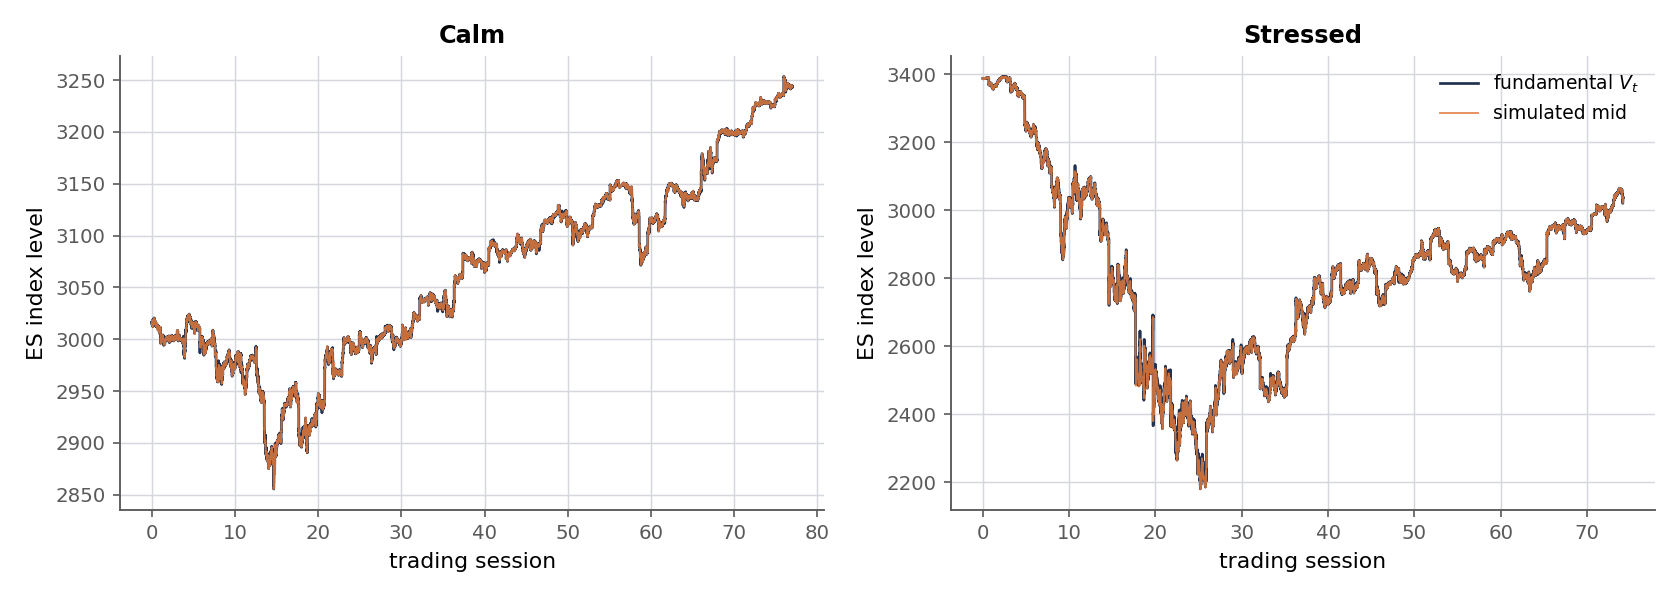
\includegraphics[width=\textwidth]{Figures/E_fv_vs_mid.png}
  \caption{\textbf{Fundamental versus simulated mid.} Empirical fundamental $V_t$ and the simulated mid
  with the clearing tier active, calm and stressed.}
  \label{fig:res-fv}
\end{figure}

\paragraph{Capital Ratios and Clearing Members.} In the stressed regime, members are pushed towards the capital-adequacy ratio of 8\% that they share. The BCMs occasionally breach and deleverage, and the NBCMs breach less often and freeze. NBCMs also sit with a higher capital ratio on average (Figure~\ref{fig:res-kappa}), but on the rare occasion where they do hit the floor and freeze, they are the only CM type that defaults. 

Each stressed seed produces an average $8.3$ client defaults (range $2$--$18$) and no defaults in calm. When the clients default, their CM seizes their IM and absorbs the remaining VM shortfall. The loss is generally contained at the CM and never reaches the default fund. In the rare case of NBCM default, 
the residual deficit it leaves --- on average
$\approx\$1.1$B --- is drawn up the waterfall: the defaulter's own default-fund contribution
($\approx\$0.11$B) and the CCP's skin-in-the-game ($\approx\$0.12$B) first, then the mutualised pooled
default fund ($\approx\$0.87$B). Against an average fund size of $\approx\$4.5$B in stress (and
$\approx\$6.3$B in calm) this draws about $19\%$ of the pooled fund.

\begin{figure}[H]\centering
  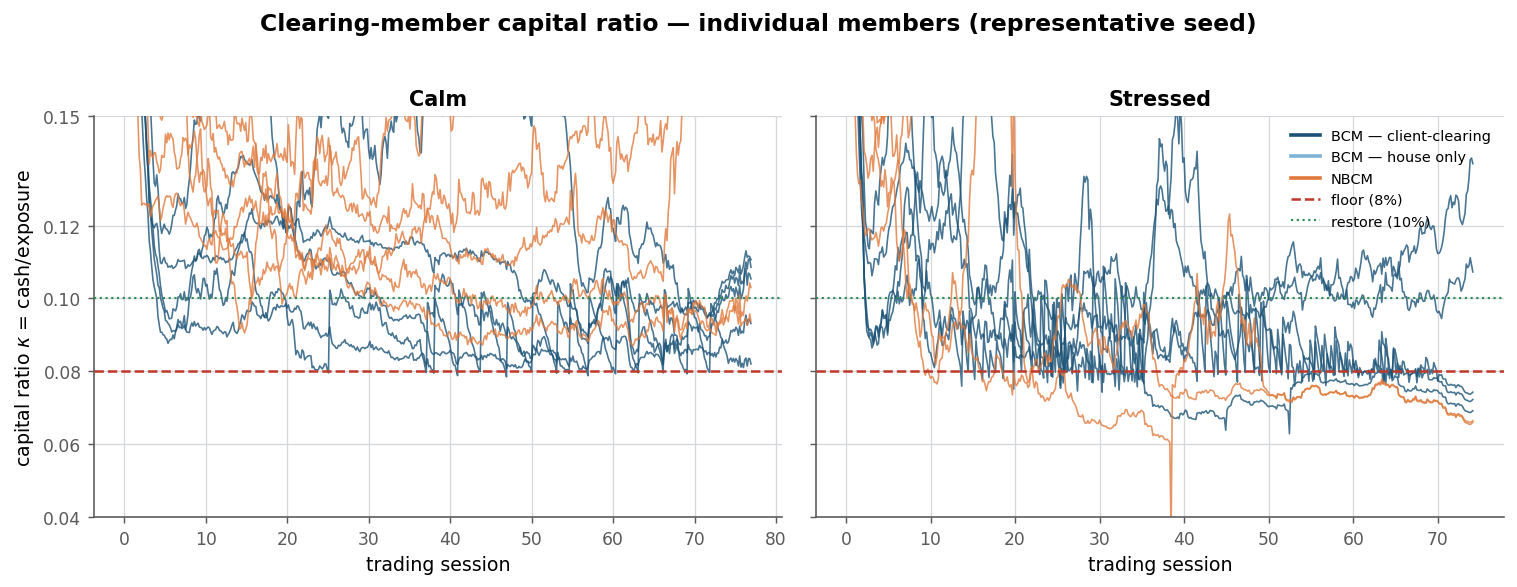
\includegraphics[width=\textwidth]{Figures/B_capital_ratio.png}
  \caption{\textbf{Clearing-member capital ratio $\kappa$.} Left: median $\kappa$ by member type over
  the stressed window (IQR band); the banks ride the $8\%$ floor (dashed) while the non-banks sit
  higher. Right: per-seed floor breaches and defaults by type --- banks breach but deleverage and
  survive, while the non-banks, unable to deleverage, are the only tier that defaults. In calm all
  members sit far above the floor.}
  \label{fig:res-kappa}
\end{figure}

\noindent This stylised result from the model stresses the importance for NBCMs to have an available external funding source that is reliable even in stressful market situations. The lack of an own book that can be liquidated to generate liquidity is a vulnerability for the NBCM, even when it freezes all client trading at a capital ratio of 8\%.

\paragraph{Margin is procyclical and clusters.} Posted margin sits at the anti-procyclicality floor of 4\% for the entirety of the calm period and the start of the stressed period, ramping up to a peak of $11.4\%$ in stressed, averaging at $7.7\%$ over the window (Figure~\ref{fig:res-im}), a result of the volatility sensitive VaR margining.

\begin{figure}[H]\centering
  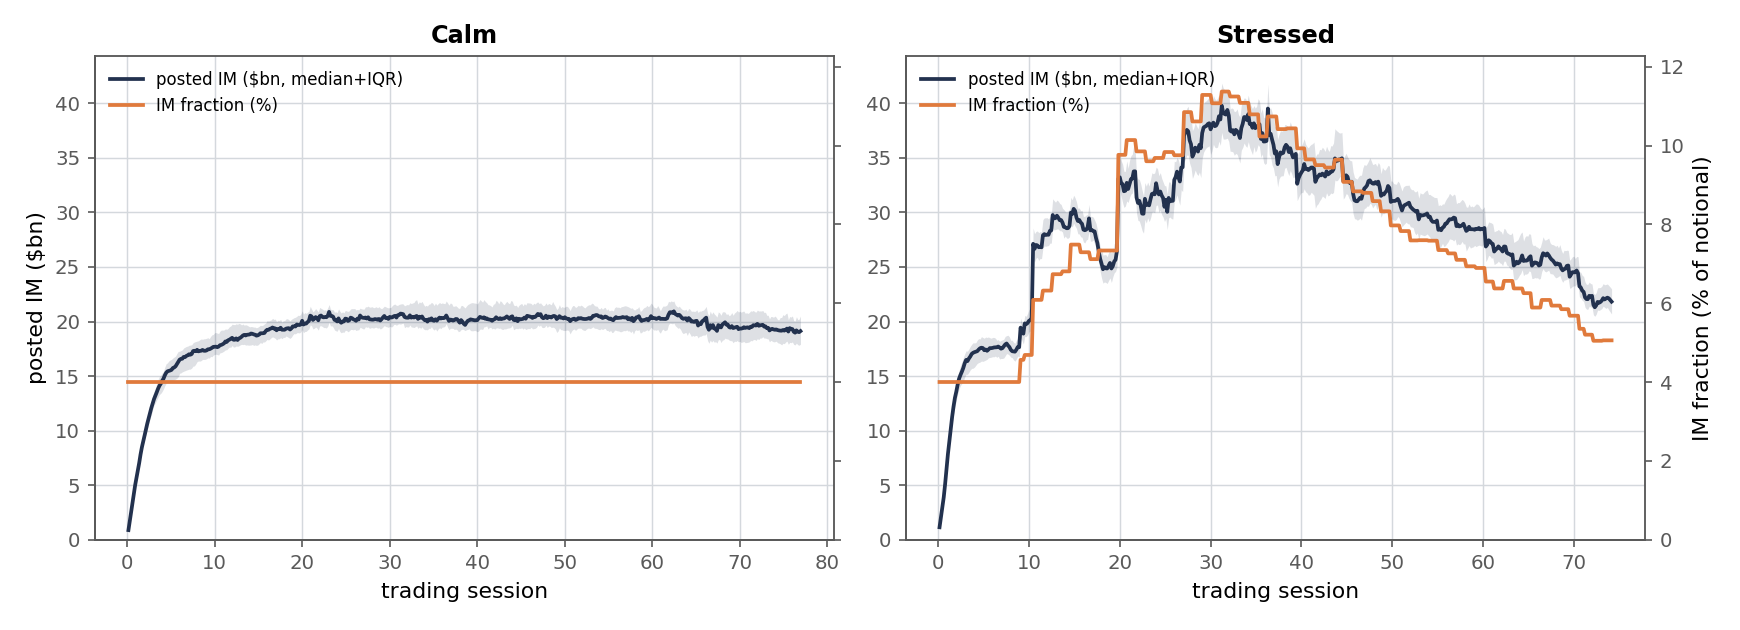
\includegraphics[width=\textwidth]{Figures/C_im_path.png}
  \caption{\textbf{Initial margin: dollar path and procyclical fraction.} Posted IM (left axis, median
  and IQR) and the charged fraction (right axis): flat at the $4\%$ floor in calm, ramping to $11.4\%$
  in stress.}
  \label{fig:res-im}
\end{figure}

\noindent Under stress, clients post roughly half of all initial margin (Figure~\ref{fig:res-imtype}). The client tier therefore has a large impact on collateral demand. We also see that FTs post the most amount of collateral, and MTs vary quite sharply in the collateral they post, a result of both higher margin requirements and increased trading in stressed markets due to their strategy and a persistent negative drawdown.

\begin{figure}[H]\centering
  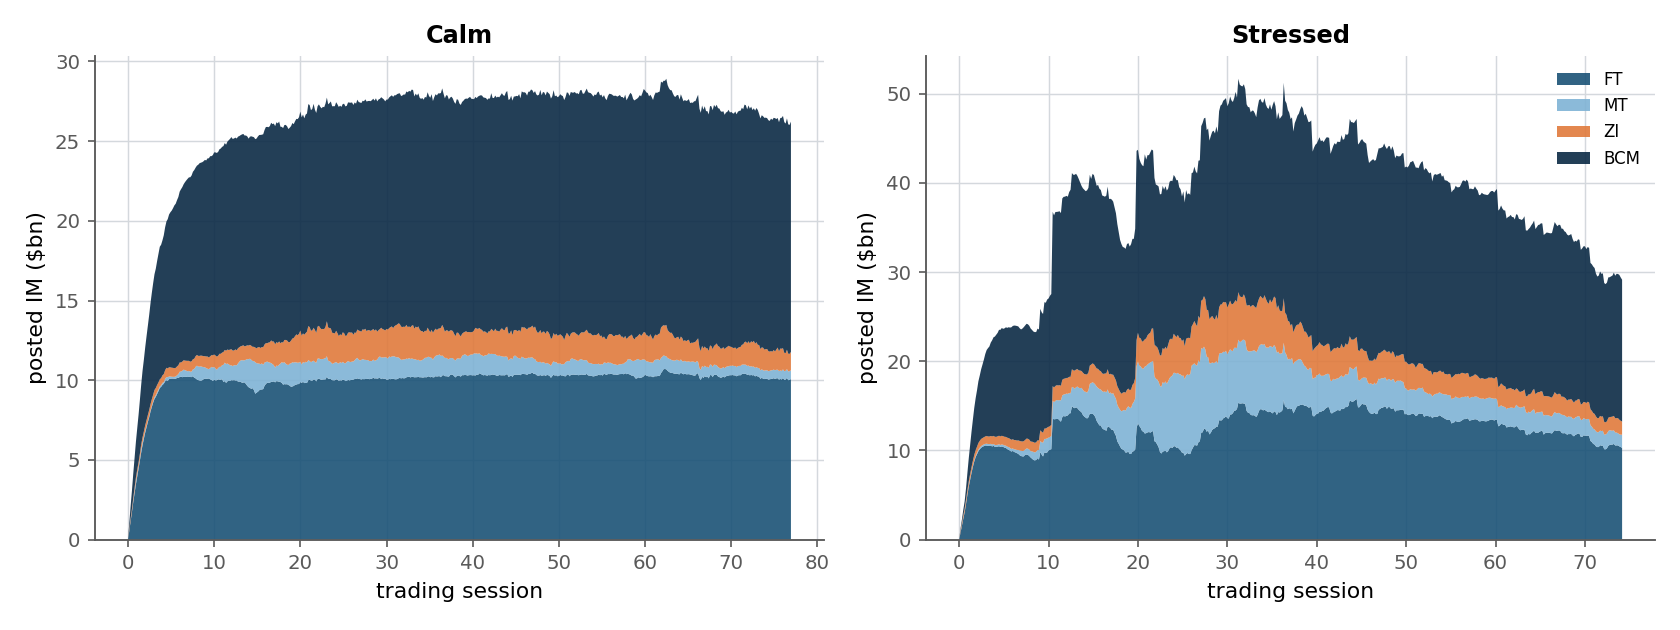
\includegraphics[width=\textwidth]{Figures/D_im_by_type.png}
  \caption{\textbf{Posted initial margin by participant type.} Fundamental, momentum and noise clients
  versus banking-member house margin; clients post about half of the total.}
  \label{fig:res-imtype}
\end{figure}

\noindent Looking at the arrival of margin calls, we see that they cluster over time, with bursts during stress (Figure~\ref{fig:res-mc}), emerging from the replicated volatility clustering in the model. This leaves CMs and clients prone to destabilising margin spikes during periods of extreme stress. 

\begin{figure}[H]
  \centering
  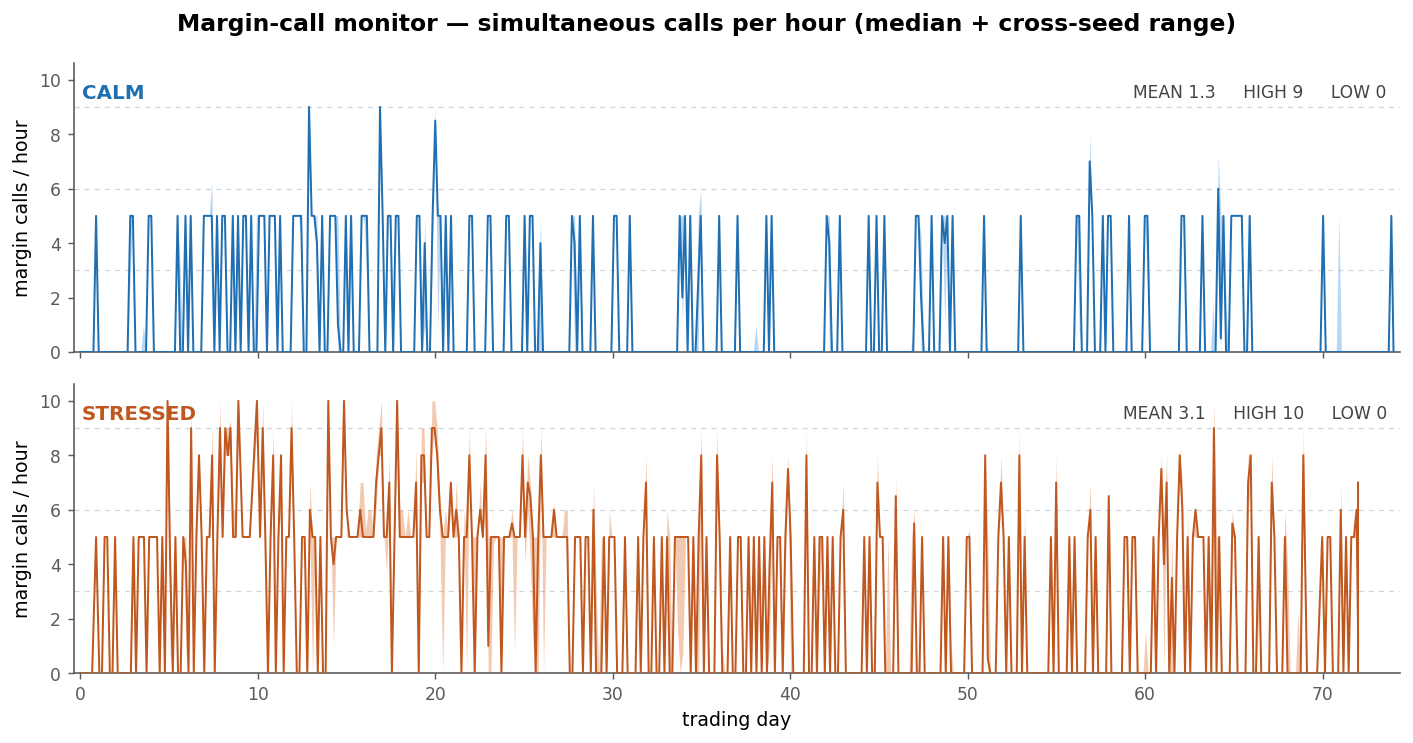
\includegraphics[width=\textwidth]{Figures/F_margin_call_clustering.png}
  \caption{\textbf{Margin-call clustering.} Margin calls per hour, calm (top) versus stressed (bottom); hours exceeding three calls are shaded. The wide, sustained bands under stress (54\% of hours) versus scattered spikes in calm (24\%) show the calls arriving in clusters rather than at random.
}
  \label{fig:res-mc}
\end{figure}

\section{Margin Procyclicality}\label{sec:resh1}

The model is then applied to look at margining practices -- volatile reactive margining is compared to flat and constant margins at different levels. Volatility sensitive margining is procyclical by construction, demanding collateral in stressful times where liquidity is hardest to raise \citep{brunnermeier_pedersen_2009,glasserman_wu_2018}. An anti-procyclicality (APC) buffer is standard practice, it asks for higher margins in calm times such that margins don't spike as much in stress. For the standard model, this was set at 4\% as covered in Section~\ref{sec:clearing-margin}. Here we look at a simple and explicit trade-off, we replace the reactive VaR margining with flat and constant margining at 3 levels -- 4\%, 8\%, and 12\%. 

The low level at 4\% is a plausible lower bound for an asset as liquid as ES futures, and is the current APC buffer in the standard model. The intermediate 8\% is close to the average margin the reactive VaR model asks for in stress times, and the high level at 12\% covers the peak of margin asked for by the model in stress. Each of these, alongside the reactive VaR margining, is run over 150 seeds and evaluated based on client defaults, member defaults, how far losses travel up the waterfall and how much it costs to post these levels of collateral.

The default fund (DF) of the standard model had to be adjusted to account for this construction. The standard model uses a Stressed-loss-over-margin to size the DF, but for the high flat IMs this often led to the DF collapsing to zero. The experiment therefore substitutes a fixed default fund, sized at $10\%$ of the two largest
members' positions (a cover-2 principle) at $\approx\$12$--$14$B --- comparable to CME Clear's --- and
applies it to both the flat and reactive arm, so that differences reflect the
margin rule alone.\\

\noindent From the results, we see that higher margin does not remove default risk but rather relocates it. As margin rises from a fixed 4\% to 12\%, client defaults fall but member defaults rise (Table~\ref{tab:res-h1}). The proportion of times the default fund is reached also rises. This happens due to a concentration of losses -- client failures become rare but also larger, falling on the member tier. The mechanism behind these is discussed further in Subsection~\ref{sec:res-mech}. While the client default decline is significant, member defaults and mutualisation are rare events and hence noisy and not statistically significant. They are, however, significant in their direction and robust to different clearing constants such as a different house capital ratio floor, default fund level and CCP recovery amount. 

\begin{table}[H]
\centering\small
\caption{\textbf{H1 --- margin regimes (stressed, 150 seeds).} Client defaults mean (sd); other columns mean
across seeds; IM in \$B; run under the ODD fixed default fund ($\approx\$12$--$14$B across arms) so the
mutualised layer is comparable. The \emph{flat ladder} reads the trade-off top-to-bottom: as the standing
margin rises, cost rises and client defaults fall, but loss climbs the waterfall (member defaults and
mutualisation rise). \emph{Reactive} (set off below) holds the flat-$4\%$ standing cost while matching
flat-$8\%$'s stress protection (its lower risk-metric means are within seed noise) --- its cost is the
stress-time \emph{peak}.}
\label{tab:res-h1}
\begin{tabular}{l cc c cc}
\toprule
 & \multicolumn{2}{c}{Cost (\$B)} & Clients & \multicolumn{2}{c}{Loss up the waterfall} \\
\cmidrule(lr){2-3}\cmidrule(lr){5-6}
Margin regime & calm & peak & client def. & member def. & reach fund \\
\midrule
Flat $4\%$    & $18.1$ & $18.6$ & $14.8\ (4.8)$ & $0.01$ & $\phantom{0}1\%$  \\
Flat $8\%$    & $31.7$ & $33.8$ & $11.1\ (4.7)$ & $0.35$ & $30\%$ \\
Flat $12\%$   & $42.3$ & $46.3$ & $\phantom{0}6.9\ (4.4)$ & $0.55$ & $42\%$ \\
\midrule
Reactive ($4\!\to\!11.4\%$) & $18.1$ & $38.5$ & $10.1\ (4.3)$ & $0.33$ & $25\%$ \\
\bottomrule
\end{tabular}
\end{table}

The attractiveness of the VaR reactive margin can be easily seen, it offers performance on risk-metrics just as well if not better than the flat 8\% margin. At the same time, it asks for a significantly lower amount of margin in calm periods and not much higher in stress (Figure~\ref{fig:res-h1}). 

\begin{figure}[H]
  \centering
  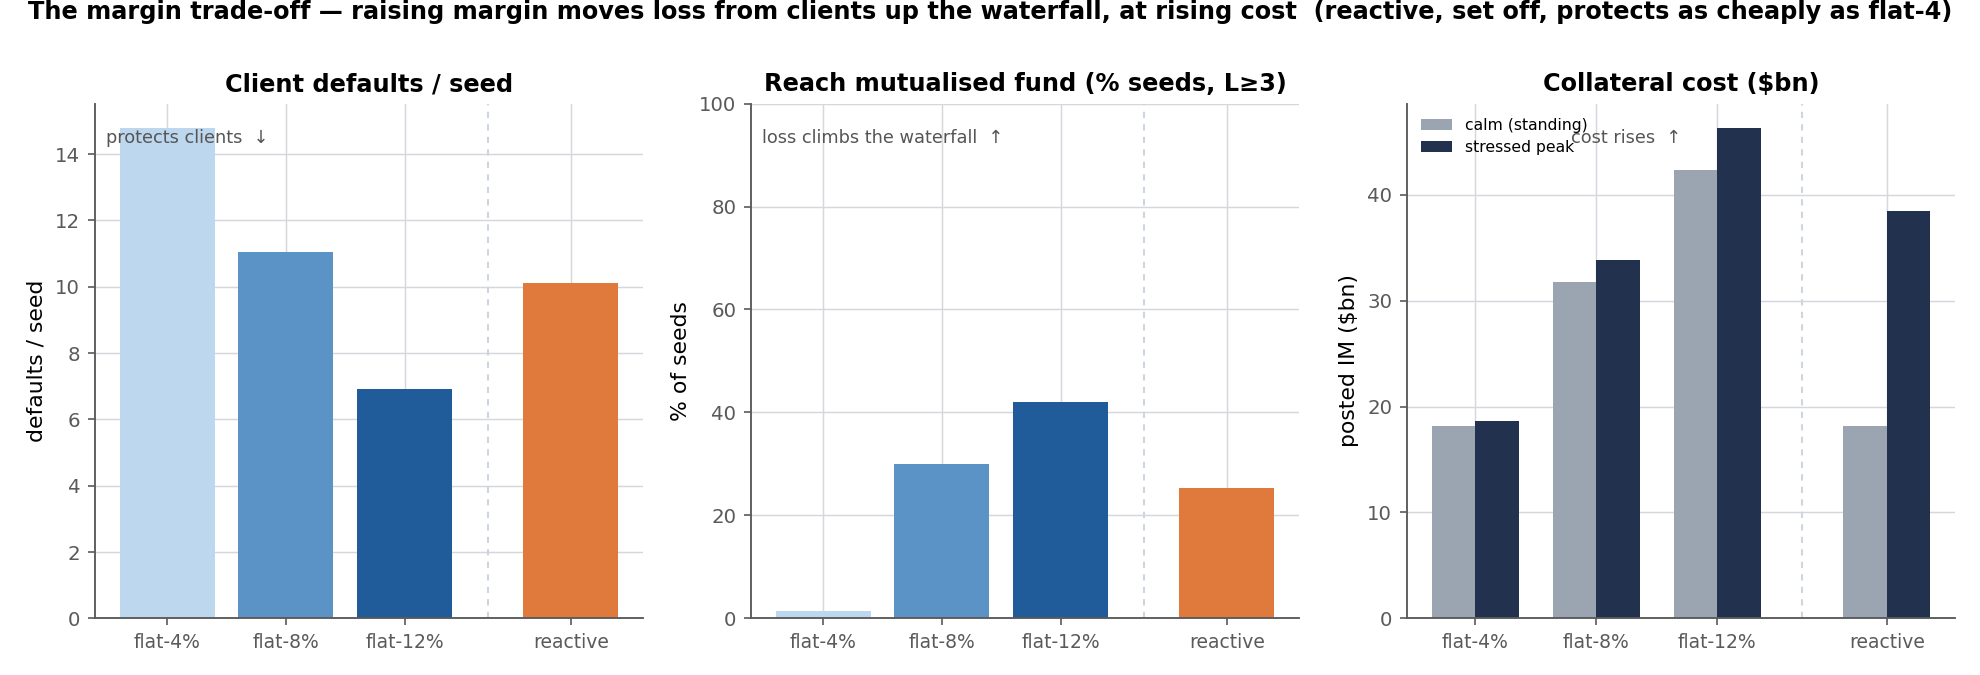
\includegraphics[width=\textwidth]{Figures/H1_margin.png}
  \caption{\textbf{H1 --- the margin trade-off.} Each panel is one outcome across the margin regimes; the
  flat ladder (light to dark) is monotonic and reactive is set off (after the dashed line) and highlighted.
  Raising the flat margin protects clients (client defaults fall, left) but pushes loss up the waterfall
  (mutualisation rises, centre) at rising standing cost (right). Reactive protects about as cheaply as
  flat-$4\%$ in calm while matching flat-$8\%$'s stress protection, paying only a stress-time peak (dark bar,
  right).}
  \label{fig:res-h1}
\end{figure}

\subsection{Mechanism: loss relocation}\label{sec:res-mech}

The relocation of defaults from clients to members as flat IM increases offers an interesting avenue for further analysis. This relocation appears to stem from CM freezes -- CMs that breach their capital adequacy floor (CAR) stop clearing, freezing their clients. The position of these clients then accumulates VM transfers due to negative returns. With higher margins, more cash is taken as margin and hence members breach their CAR earlier in the crash, but at the same time, this turns into a trap. Due to the early freeze, clients holding onto a large position cannot liquidate it and default as the market falls. Despite the median of defaulted positions being lower for higher flat margins, the tail of positions on default is a lot higher (Figure~\ref{fig:mech-position}). The member then assumes this large position that it must liquidate onto a falling market, and the losses on this overwhelm especially the NBCMs causing them to default. 

\begin{figure}[H]\centering
  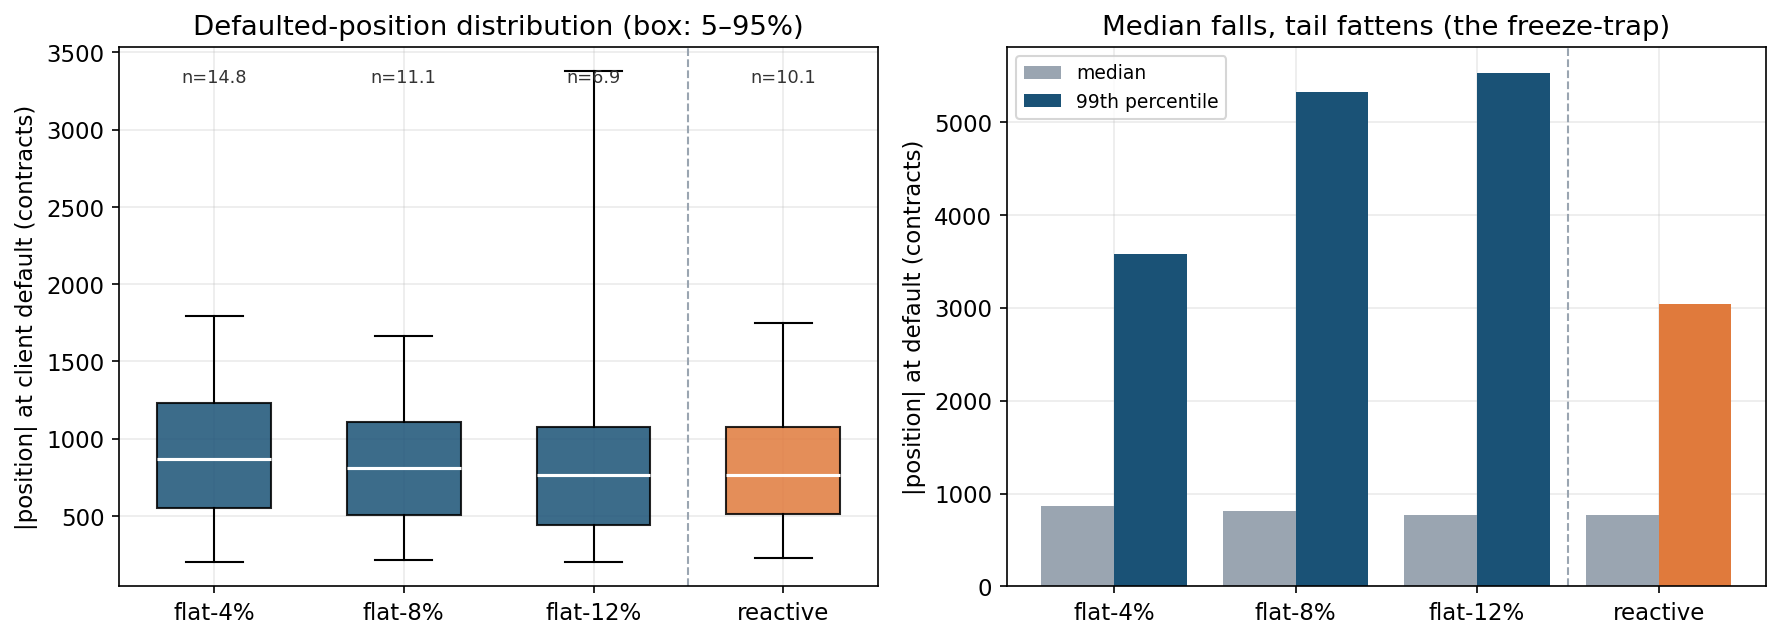
\includegraphics[width=\textwidth]{Figures/mech_position.png}
  \caption{\textbf{The freeze-trap.} Distribution of $|$position$|$ at client default by margin regime
  (left; box spans $5$--$95\%$, $n=$ defaults per seed) and the median versus the $99$th percentile
  (right). Higher flat margin yields fewer, smaller-median defaults but a fatter tail; reactive keeps
  the tail thin.}
  \label{fig:mech-position}
\end{figure}

\noindent This highlights the vulnerability these clients face by having only a single clearing connection at the mode \citep{ofr_2026}. If a CM facing capital or liquidity constraints decides to freeze offering clearing services to its clients, the clients are left holding onto a possible unwanted position that by regulation must be centrally cleared. At the same time, this is also a consequence of the simplified model design. In reality, an inability to liquidate is not an absolute, but in stressed market situations, porting and finding new members would prove to be difficult. \cite{acosta_smith_2018} also show that capital ratio requirements did leave members less willing to provide clearing services.  


\section{A Synthetic Path Alternative}\label{sec:res-synth}

So far, the results replay a historical period, using the empirical mid price as a Fundamental Value. This creates a natural limitation for this model - it can only be simulated over one path. This section provides an alternative, switching out the FV for a stochastic and synthetic series that reproduces the same stylised facts seen in the stressed period. The parameters of the synthetic FV are then calibrated jointly with agent parameters to reproduce stressed empirical moments, with the calibration yielding a fit in stress near identical to the empirical path, with moments such as volatility clustering being better reproduced (Section~\ref{sec:cal-synth}). The simulation is then run on 80 seeds, yielding 80 different paths for the Fundamental Value, and hence also for the simulated mid. The drift of these paths is similar to the COVID stressed window, but the stochastic runs yield both less and more extreme paths (Figure~\ref{fig:synth-paths}), which makes it well suited to studying CCP resilience across many stress scenarios.

\begin{figure}[H]
  \centering
  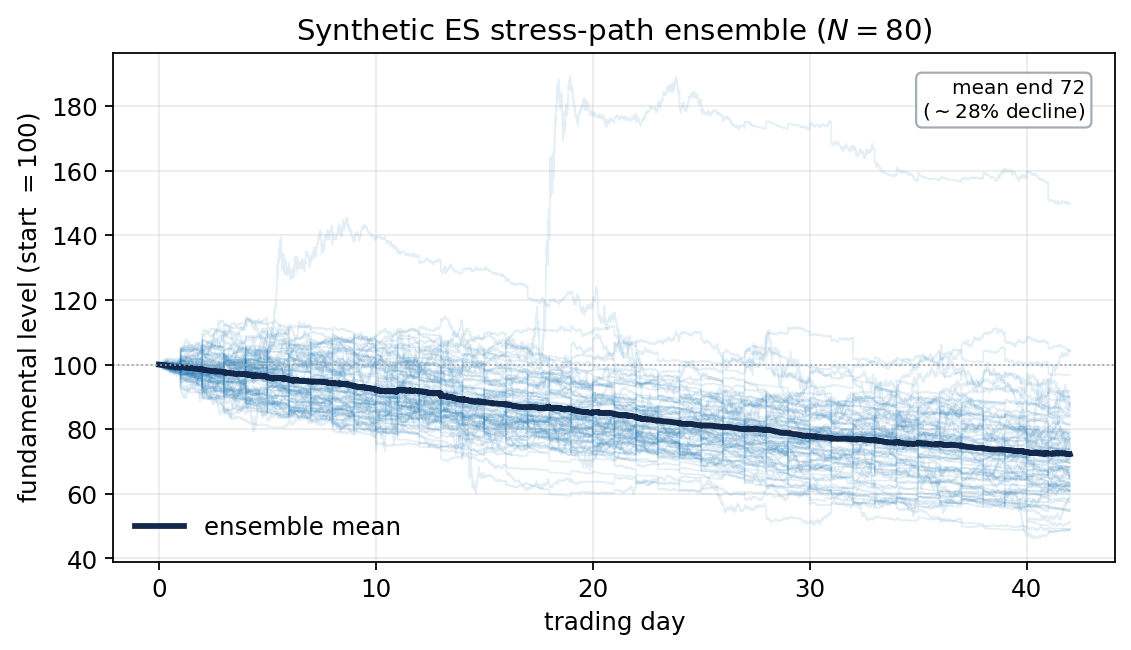
\includegraphics[width=0.72\textwidth]{Figures/synth_paths.png}
  \caption{\textbf{Synthetic two-factor-SV stress-path ensemble.} $N=80$ independent synthetic ES fundamental
  paths (thin) with the ensemble mean (bold), drifting down at the stressed-window rate.}
  \label{fig:synth-paths}
\end{figure}

\paragraph{A tail within a tail.} A point to note is that these paths are already based on a stressed environment, one that would form the tail of any normal distribution. The median path here is hence already a tail path. We see that despite this, for the median path, there are only 3 client defaults, no member defaults, and the default fund is never drawn (Table~\ref{tab:synth-clearing}). Across 80 such extreme paths, only 14 reach the mutualised default fund in this stylised model. 

\begin{table}[H]
\centering\small
\caption{\textbf{Clearing outcomes across the $N{=}80$ synthetic stressed ensemble} (reactive margining,
$42$-day paths). Posted initial margin in \$B; the waterfall levels L1--L5 follow the model's five-level
default waterfall (L3 the mutualised default fund, L4 surviving-member loss-sharing, L5 CCP capital).}
\label{tab:synth-clearing}
\begin{tabular}{lccc}
\toprule
 & Median path & Ensemble mean & Worst path \\
\midrule
Client defaults          & $3$    & $7.8$  & $68$   \\
Member defaults          & $0$    & $1.0$  & $15$   \\
Peak posted IM (\$B)     & $43.5$ & $44.7$ & $80.8$ \\
Deepest waterfall level  & $0$    & ---    & $5$    \\
\midrule
\multicolumn{4}{l}{\footnotesize $14/80$ paths reach the mutualised default fund (L$\geq3$); $8$ reach
member loss-sharing (L4); $3$ reach CCP cash (L5).}\\
\bottomrule
\end{tabular}
\end{table}

\paragraph{Volatility and drawdowns.} Looking at the paths by realised volatility, the first two-thirds are benign. There are around 3 client defaults per path, no member defaults and the default fund isn't breached. The defaults and stress are concentrated in the bottom third. Interestingly, the median drawdown of the paths that breach the DF is $29\%$, lower than the median $35\%$ of the paths that never breach. Furthermore, the clearing outcomes carry a robust rank correlation with realised volatility (Spearman
$\rho\approx0.5$, $p<0.001$, $n=80$) but none with the net drawdown. This can perhaps be explained by the margin mechanism, VM simply transfers from one member to another and is redistributed. IM, on the other hand, drains the balance of all members (Figure~\ref{fig:synth-clearing}). This rises with volatility, and offers an insight into just how draining IM can be with VaR margin models. 


\begin{figure}[H]
  \centering
  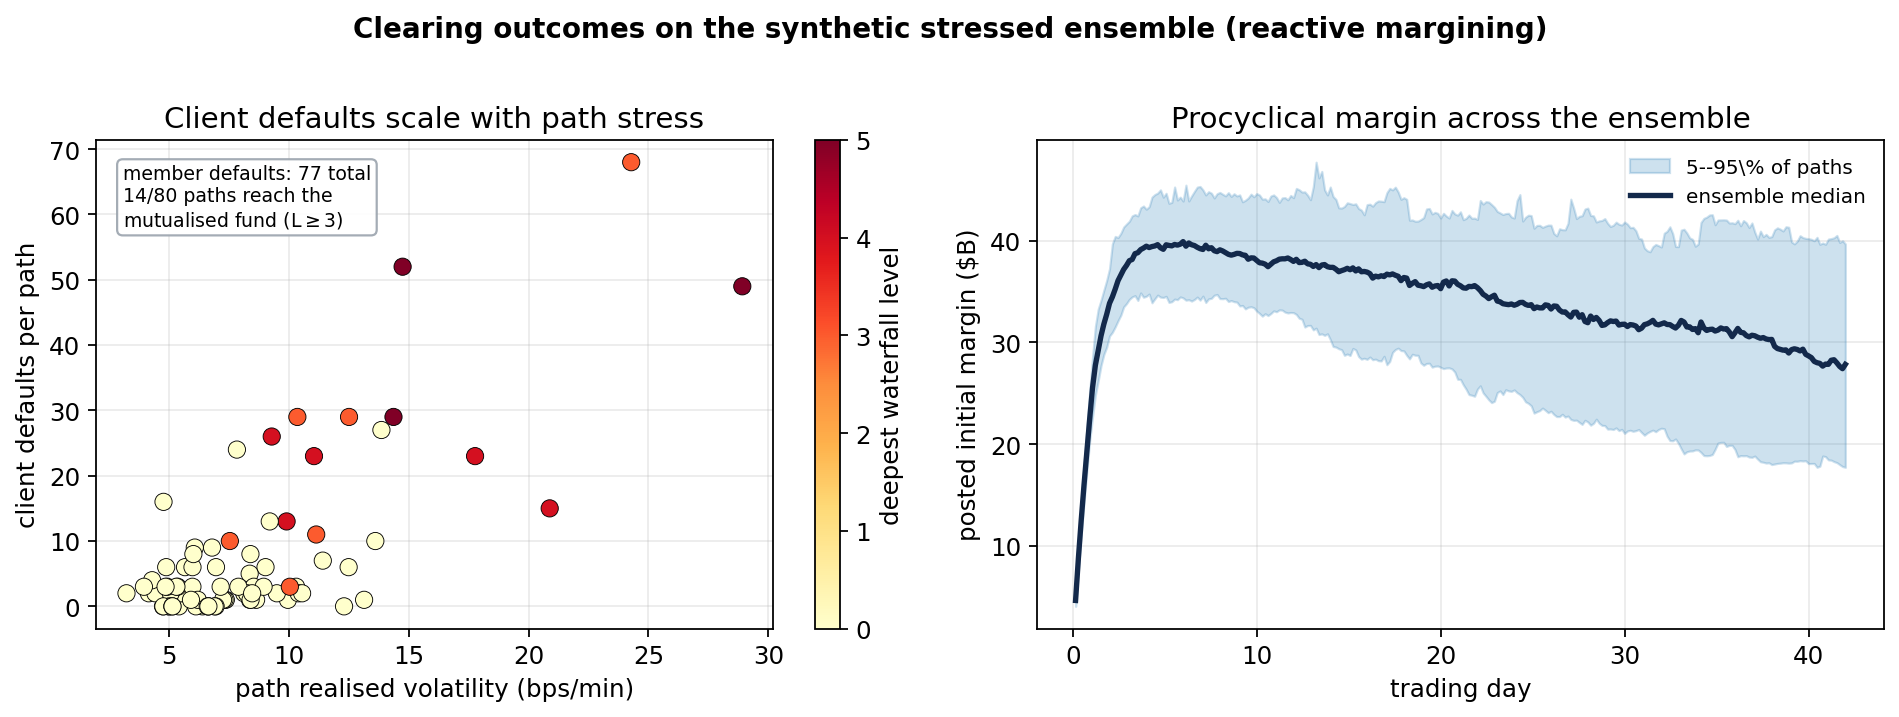
\includegraphics[width=\textwidth]{Figures/synth_clearing.png}
  \caption{\textbf{Clearing on the synthetic stressed ensemble.} Left: per-path clearing stress (client
  defaults) against the path's realised volatility, coloured by the deepest waterfall level reached and sized
  by member defaults. Right: posted initial margin over the window (ensemble median and $10$--$90\%$ band) --- the
  procyclical ramp is consistent across all $80$ paths, while within a path the calls themselves cluster in
  time.}
  \label{fig:synth-clearing}
\end{figure}

Overall, the member tier can absorb defaults across the median stressed paths. The extreme paths, however, do push the CCP to its limits, exhausting default funds and tapping into member cash reserves. While the model is a definite simplification, and some results may emerge as a consequence of model design over being an accurate representation of society, its ability to simulate outcomes across various paths, studying the effects of changes in various parameters and CCP recovery practices offers a definite benefit.  

% \chapter{Implications}\label{ch:implications}
% \input{chapters/06_implications}

% \chapter{Conclusion}\label{ch:conclusion}
% \input{chapters/07_conclusion}

% ------------------------------------------------
% References
% ------------------------------------------------
\clearpage
\bibliographystyle{apalike}   
\bibliography{references}

% ------------------------------------------------
% Appendices
% ------------------------------------------------
\appendix

\chapter{Additional Tables and Figures} \label{ch:appendix}
\section{Market Microstructure}\label{app:microstructure}
The calibrated market layer's microstructure, summarised in Section~\ref{sec:res-general}, is shown in
full here. Traded volume rises under stress and the book thins and skews to the sell side
(Figure~\ref{fig:app-flow}); the resting bid/ask depth profile is in Figure~\ref{fig:app-depth}.

\begin{figure}[H]\centering
  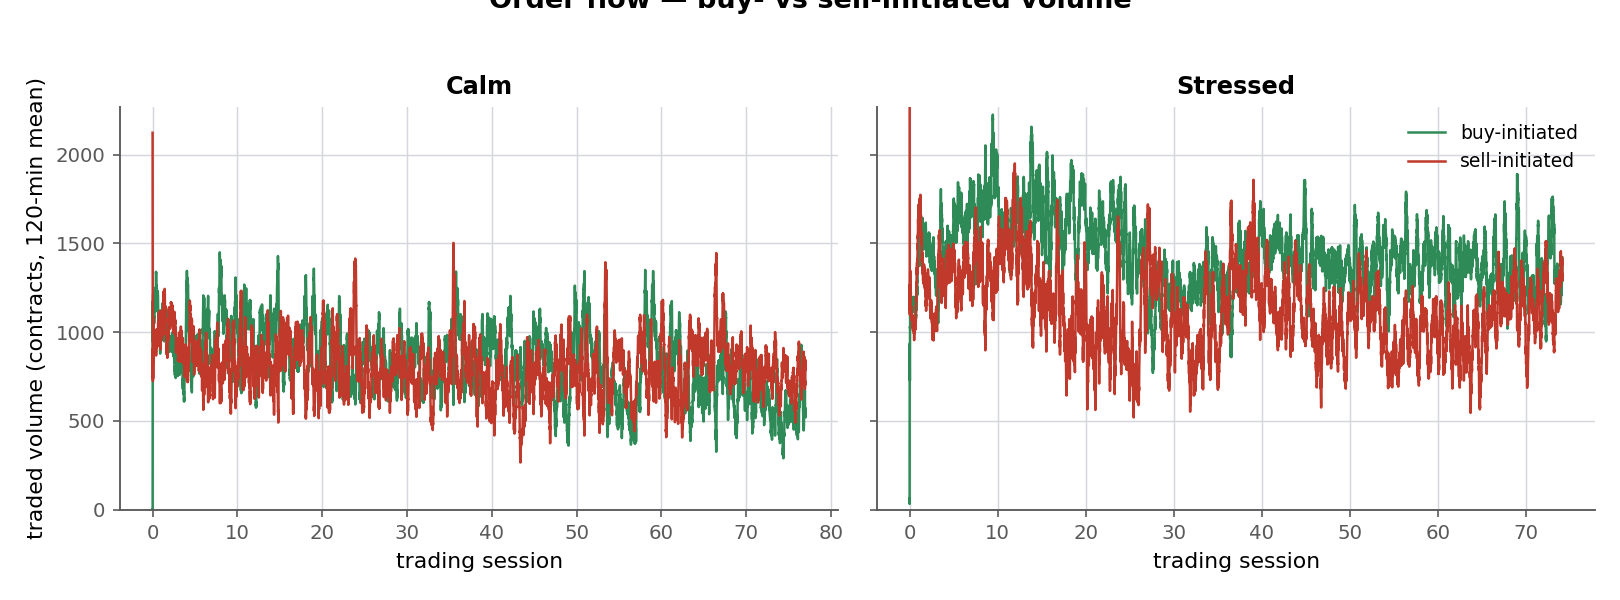
\includegraphics[width=\textwidth]{Figures/A_order_flow.png}
  \caption{\textbf{Order flow.} Buy- versus sell-side activity, calm versus stressed.}
  \label{fig:app-flow}
\end{figure}

\begin{figure}[H]\centering
  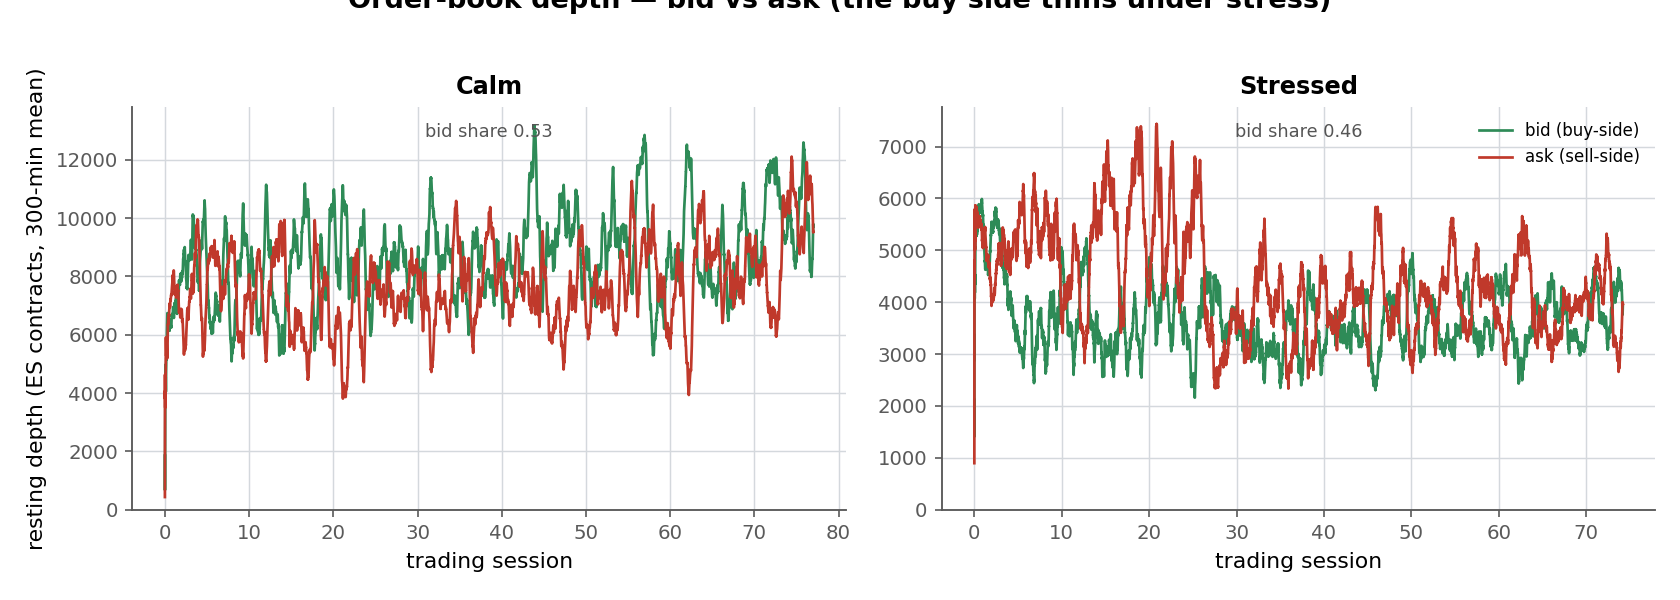
\includegraphics[width=\textwidth]{Figures/A2_book_depth.png}
  \caption{\textbf{Order-book depth.} Bid versus ask resting depth, calm versus stressed.}
  \label{fig:app-depth}
\end{figure}


\end{document}

